\section{Mass-spring-damper System}

\begin{figure}[h]
    \centering
    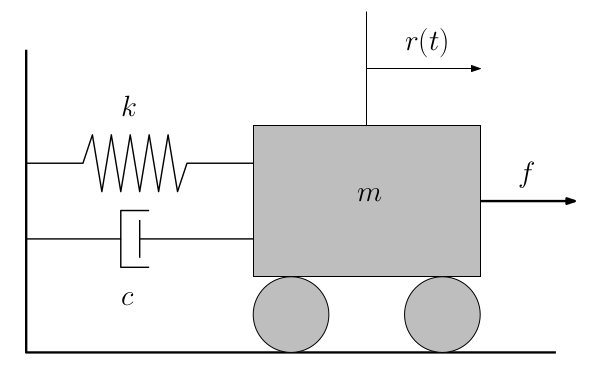
\includegraphics[width=0.6\textwidth]{figures/mass_spring_damper.png}
    \caption{Mass-spring-damper system.}
    \label{fig:mass_spring_damper}
\end{figure}

Figure~\ref{fig:mass_spring_damper} shows a mass-spring-damper system, 
consisting of a mass \( m \) attached to a spring with spring constant \( k \), 
a dashpot with damping constant \( c \), and also subject to an external force \( f(t) \). 
The position of the cart from its equilibrium position is denoted as \( r(t) \), 
which is a function of time \( t \).

The equation of motion of the cart is given by

\begin{align}
    \ddot{r}(t) + c\dot{r}(t) + kr(t) = f(t)
\end{align}
\clearpage

\subsection{No external Force}

With no external force, the equation of motion becomes

\begin{align}
    \ddot{r}(t) + c\dot{r}(t) + kr(t) = 0 \\
    \ddot{r}(t) = \frac{1}{m}(-k r(t) - c \dot{r}(t))
\end{align}

The state-space form is given by
 
\begin{equation}
    \begin{aligned}
        \dot{\mathbf{x}}(t) &= 
        \begin{bmatrix}
            0 & 1 \\
            -\dfrac{k}{m} & -\dfrac{c}{m}
        \end{bmatrix}
        \mathbf{x}(t), \quad\quad
        \mathbf{x}(t) = 
        \begin{bmatrix}
            r(t) \\
            \dot{r}(t)
        \end{bmatrix}
    \end{aligned}
    \end{equation}

\subsection{Non-zero external Force}

Let \( f(t) = A \sin(\omega t) \), the equation of motion becomes:

\begin{align}
    \ddot{r}(t) + c\dot{r}(t) + k r(t) = A \sin(\omega t)
\end{align}

The state-space form is given by
    
\begin{equation}
    \begin{aligned}
        \dot{\mathbf{x}}(t) &= 
        \begin{bmatrix}
            0 & 1 \\
            -\dfrac{k}{m} & -\dfrac{c}{m}
        \end{bmatrix}
        \mathbf{x}(t) + 
        \begin{bmatrix}
            0 \\
            -\dfrac{1}{m}
        \end{bmatrix}
        \mathbf{u}(t), \quad\quad
        \mathbf{x}(t) = 
        \begin{bmatrix}
            r(t) \\
            \dot{r}(t)
        \end{bmatrix}, \;
        \mathbf{u}(t) = A sin(wt)
    \end{aligned}
    \end{equation}
    